\graphicspath{{chapters/04/images/}}
\chapter{Approximation algorithms}

\section{Introduction}
Exact simulation of complex biological system is often to expensive due to their stochastic and multi scale nature.
These lead to the development of approximate algorithms, which improve the simulation efficiency by sacrificing their accuracy.
Multiple firings are coalesced and performed together in one simulation step with a huge speed up.
Approximate methods should be used because:

\begin{multicols}{2}
  \begin{itemize}
    \item It might be the only possible and feasible solution to solve a problem.
    \item reality is affected by error, so even when using exact stochastic simulation algorithms a small degree of approximation should be considered.
      A certain deal of error could aid in retrieving a more realistic result.
  \end{itemize}
\end{multicols}

In this case, each algorithm (Figure \ref{fig:SSA_tree}) approximates in a different way,  assuming different approximations.
Of the three main computational strategies presented here, there is one which is much more popular with respect to the others the $\tau$ leaping method.

\begin{figure}]H]
  \centering
  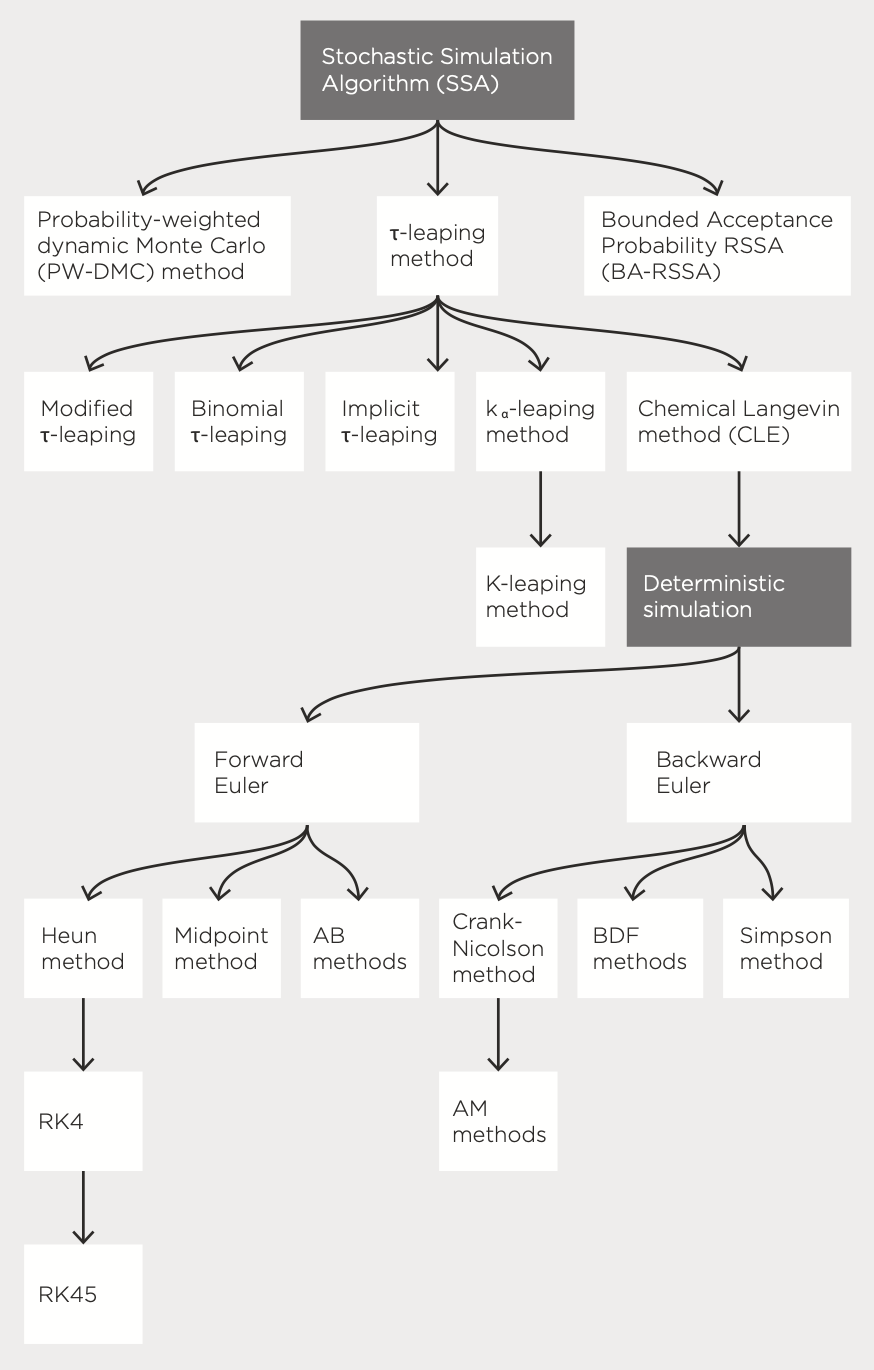
\includegraphics[width=\textwidth]{SSA_tree.png}
  \caption{Relationship between stochastic simulation algorithms}
    \label{fig:SSA_tree}
\end{figure}


To improve the exact simulations algorithms, one should consider to:

\begin{multicols}{2}
  \begin{itemize}
    \item Work on the number of reaction events, grouping them in such a way to reduce the number of reactions in the system.
      The $\tau$ leaping methodology is working in this direction.
    \item Improve the computation of the propensity.
      For instance, the probability-weighted Monte Carlo is particularly promising in situations in which there is a huge differences in propensities among reactions.
  \end{itemize}
\end{multicols}

\section{Probability-Weighted Dynamic Monte Carlo Method}
The probability-weighted dynamic Monte Carlo method (PW-DMC) is an approximation approach for improving the computational efficiency of stochastic simulations of reaction networks where some reactions have propensities significantly larger than other reactions.
This is because fast reactions (with large propensities) occur frequently and dominate the simulation, while slow reactions (with small propensities) occur less frequently.
The events from the slow reaction are rare and their statistical estimation is unreliable.
PW-DMC attempts to equalize the propensities of reactions so that a larger increment time step can be chosen, improving simulation's performance.

  \subsection{Weighted sampling}
  The principle of this algorithm is a sort of modification of the probability distribution of the next reaction firing through weighted sampling.
  The propensity $a_j$ of $R_j$ is scaled by a biasing weight $w_j$ defined as the number of firing of $R_j$ at each step.
  To compute it the unweighted probability $\frac{a_j}{a_0}$ is discretized into integer valued histogram bins according to a size $b$.

    \subsubsection{Effective propensity}
    The effective propensity $a^w_j$ is computed as:

    $$a^w_j = \frac{a_j}{w_j}$$

    These are then used for the selection of $R_\mu$.
    The chance that a slow reaction fires is increased and so is the frequency of rate events.

  \subsection{Realization of the reaction firing}
  The realization of the next reaction firing has two step:

  \begin{multicols}{2}
    \begin{itemize}
      \item Selection of the reaction.
      \item Correction of the firing time.
    \end{itemize}
  \end{multicols}

    \subsubsection{Selection of the reactoin}
    $R_\mu$ is selected with probability $\frac{a_\mu^w}{a_0^\mu}$, where $a_0^\mu = \sum\limits_{j=1}^Ma_j^w$.
    This can be done by linearly accumulating $a_\mu^w$ as:

    $$\mu = \arg\min\limits_{j\in \mu}\sum\limits_{j=1}^\mu a_j^w\ge r_1a_0^w$$

    Where $r_1\sim norm(0,1)$.

    \subsubsection{Correction of the firing time}
    The firing time $\tau$ is corrected to account for the bias.
    $\tau$ is generated from an exponential distribution with rate $a_0^w$:

    $$\tau = \frac{1}{a_0^w}\ln\left(\frac{1}{r_2}\right)$$

    Where $r_2\sim norm(0,1)$.
    Then the state at time $t+\tau$ is updated assuming there are $w_\mu$ consecutive firings of $R_\mu$ in $[t,t+\tau[$ ant the state at time $t+\tau$ is updated as:

    $$X(t+\tau) = X(t) + w_\mu\vec{v}_\mu$$

    The weight of the reactions have to be updated accordingly.

  \subsection{Bounds on the weights}
  $w_j$ should be an integer value because the population of a species involved in a reaction is an integer.
  Its magnitude is constrained in order to bound the error in the results.
  Each time $R_j$ is selected it fires $w_j$ times.
  The change of each species $S_i$ in $R_j$ is $w_j$, the fluctuation of the population is thus $\frac{w_j}{X}$.
  This ratio must be less than a predefined tolerance $\epsilon$ to ensure the statistical uncertainty of the estimation of $X_i$.
  Moreover the ration would be negligibly small when the population of species is large, and the chosen weight does not affect the simulation result.
  However the weight introduces an approximation to the temporal dynamics when the population of species is low and in this case $w_j$ must be adjusted to maintain $w_j< \epsilon X_i$.

  \subsection{Algorithm}
  An implementation of PW-DMC can be found in algorithm \ref{algo:pw-dmc}.

  \begin{algorithm}[H]
\DontPrintSemicolon
\SetKwComment{comment}{$\%$}{}
\SetKw{Int}{int}
\SetKw{To}{to}
\SetKw{Return}{return}
\SetKw{Not}{not}
\SetKw{Input}{Input}
\SetKw{Output}{Output}
\SetKwData{Item}{item}
\SetKwFunction{Min}{min}
\SetKwFunction{TitleFunction}{Probability-Weighted Dynamic Monte Carlo (PW-DMC)}

\caption{\protect\TitleFunction{}}
\label{algo:pw-dmc}

\Input: a biochemical reaction network of $M$ reactions in which each reaction $R_j$, $j=1, \dots, M$ is accompanied with the state change vector $\vec{v}_j$ and the propensity $a_j$, the initial state $\vec{x}_0$ at time $0$ and the simulation ending time $T_{\max}$, the size $b$ for discretizing probability of reacitons and tolerance $\epsilon$ for constraining the fluctuation of species.\;

\Output: a trajectory of the biochemical reaction network, which is a collection of states $X(t)$ for time $0\le t\le T_{\max}$\;

$t = 0$\;
$\vec{X} = \vec{x}_0$\;
build the reaction dependency graph $G$\;
compute propensity $a_j$ for each reaction $R_j$\;

\While{$t<T_{\max}$}{
	compute $w_j$ for each $R_j$\;
	compute $a_j^w = \frac{a_j}{w_j}$ for each $R_j$\;
	$a_0^w = \sum\limits_{j=1}^Ma_j^w$\;
	generate two random numbers $r_1, r_2\sim norm(0,1)$\;
	select $R_\mu$ with the smallest index $\mu$ such that $\sum\limits_{j=1}^\mu a^w_j\ge r_1a^w_0$\;
	$\tau = \frac{1}{a^w_0}\ln\frac{1}{r_2}$\;
	$\vec{X} = \vec{X}+w_\mu\vec{v}_\mu$\;
	$t=t+\tau$\;
	\ForEach{$R_j\in Dependents(R_\mu)$}{
		update $a_j$\;
	}
}

\end{algorithm}


  \subsection{Discussion}

    \subsubsection{Time complexity}
    The speed-up gain in PW-DM is achieved by multiple firings of a reaction in each step.
    The weight can be tuned to produce a significant gain in computational performance, while keeping accuracy.
    The frequency of rare events is increased, helping explore more the biochemical systems.

    \subsubsection{Limitations}
    PW-DMC skews the probability distribution of the state, because the weight sampling groups reaction of the same type in bundles and fires them together, loosing the order of reaction.
    PW-DMC could misdescribe the fluctuation of species in the result.
    $\epsilon$ has to be set for constraining fluctuation of species to a reasonably small value in order to bound the accuracy of the simulation.

\section{Bounded acceptance probability RSSA}
The bounded acceptance probability RSSA BA-RSSA focuses on the simulation of reactions involved species with both small and large population.
These will have a large propensity.
Many firings can occur in time interval and quickly deplete the small population species.
To bound the error updates must be performed frequently, degrading the simulation performance, especially if the small population is a hub species.
The simulation of this reactions is accelerated by bounding the acceptance of a candidate reaction selected by RSSA.
It accepts a candidate reaction without validation if its acceptance probability is greater than a user-defined probability, reducing the computational cost for both selecting of reaction firing and propensity updates.

  \subsection{Defining the bounds}
  Let $0\le\alpha\le 1$ be a constant defined as a lower bound for the acceptance probability and $R_j$ the selected reaction.
  BA-RSSA guarantees that the probability that $R_j$ is accepted to fire is greater than $\alpha$.
  The validation step of standard RSSA accepts $R_j$ to fire with probability $\frac{a_j(X(t))}{\overline{a_j}}$, the goal of BA-RSSA is to ensure:

  $$\frac{a_j(X(t))}{\overline{a_j}} \ge \alpha$$

  This is difficult to assess because it depends on $X(t)$.
  Anytime the state changes $a_j$ has to be re-evaluated.
  To cope with this BA-RSSA exploits the fact that $a_j(X(t))\ge \underline{a_j}$ when $X(t)\in[\underline{X}, \overline{X}]$, therefore if:

  $$\frac{\underline{a_j}}{\overline{a_j}}\ge \alpha$$

  Holds for each reaction $\frac{a_j(X(t))}{\overline{a_j}} \ge\alpha$ is automatically satisfied.

  \subsection{Defining the fluctuation interval}
  To enforce $\frac{\underline{a_j}}{\overline{a_j}}\ge \alpha$, $[\underline{X}, \overline{X}]$ has to be defined so that $\frac{\underline{a_j}}{\overline{a_j}}$ of each $R_j$ within the fluctuation interval is bounded by $\alpha$.
  A fluctuation rate $\delta_i$ for each $S_i$ involved in $R_j$ has to be selected so that when $S_i$ fluctuates in $[(1-\delta_i)X_i(t), (1+\delta_i)X_i(t)]$ the inequality is satisfied.
  Only a range of $\delta_i$ can be chosen given the ratio of propensity bounds.

    \subsubsection{Computing the maximum fluctuation rate}
    The maximum fluctuation rate $\delta_i$ computation is reaction dependent.

      \paragraph{Synthesis reaction}
      For a synthesis reaction $R_j$, $a_j$ is independent of $X(t)$ and is equal to $x_j$.
      Also the bounds are constant, the ratio is equal to $1$ and the inequality is satisfied.

      \paragraph{Unimolecolar reaction}
      For a unimolecular reaction $R_j$, $\overline{a_j} = c_j(1+\delta_i)X_i$ and $\underline{a_j} = c_j(1-\delta_i)X_i$, so that the inequality becomes:

      $$\frac{1-\delta_i}{1+\delta_i}\ge\alpha$$

      The maximum value of $\delta_i$ then becomes:

      $$\delta_i = \frac{1-\alpha}{1+\alpha}$$

      \paragraph{Bimolecular reaction}
      For a bimolecular reaction $R_j$ $\overline{a_j} = c_j(1+\delta_j)(1+\delta_k)X_iX_k$ and $\underline{a_j} = c_j(1-\delta_i)(1-\delta_k)X_iX_k$, so that:

      $$\frac{(1-\delta_i)(1-\delta_k)}{(1+\delta_i)(1+\delta_k)}\ge \alpha$$

      Which is a quadratic equation of two independent variables, which can be splitted in to part so that:

      $$\frac{1-\delta_i}{1+\delta_i}\ge\sqrt{\alpha}\land\frac{1-\delta_k}{1+\delta_k}\ge\sqrt{\alpha}$$

      So that the maximum values for the fluctuation rates are:

      $$\delta_i = \delta_k = \frac{1-\sqrt{\alpha}}{1+\sqrt{\alpha}}$$

      \paragraph{Dimerization reaction}
      For a dimerization reaction $R_j$ by a similar derivation as the bimolecular one:

      $$\frac{(1-\delta_i)((1-\delta_i)X_i-1)}{(1+\delta_i)((1+\delta_i)X_i-1)}\ge\alpha$$

      So that the maximum $\delta_i$:

      $$\delta_i = \frac{1-\sqrt{\alpha}}{1+\sqrt{\alpha}}\left(1-\frac{1}{X_i}\right)$$

  \subsection{Selecting the propensity}
  Once the state is confined in a fluctuation interval that satisfies the bounds, any $b_j\in[\underline{a_j}, \overline{a_j}]$ can be chosen as the propensity.
  The extreme values may bias the selection step, so the average can be used:

  $$b_j = \frac{\underline{a_j}+\overline{a_j}}{2}$$

  This choice requires two evaluation of the propensity function.
  Another choice is to compute the value of the propensity at the central point of the fluctuation interval so to have one evaluation of the propensity function:

  $$b_J = a_j\left(\frac{\underline{X}+\overline{X}}{2}\right) = a_j(X(t))$$

  \subsection{Algorithm}
  An implementation of BA-RSSA can be found in algorithm \ref{algo:ba-rssa}.

  \begin{algorithm}[H]
\DontPrintSemicolon
\SetKwComment{comment}{$\%$}{}
\SetKw{Int}{int}
\SetKw{To}{to}
\SetKw{Return}{return}
\SetKw{Not}{not}
\SetKw{Input}{Input}
\SetKw{Output}{Output}
\SetKw{False}{false}
\SetKw{True}{true}
\SetKwData{Item}{item}
\SetKwFunction{Min}{min}
\SetKwFunction{TitleFunction}{Buonded Acceptance Probability RSSA (BA-RSSA)}

\caption{\protect\TitleFunction{}}
\label{algo:ba-rssa}

\Input: a biochemical reaction network of $M$ reactions in which each reaction $R_j$, $j=1, \dots, M$ is accompanied with the state change vector $\vec{v}_j$ and the propensity $a_j$, the initial state $\vec{x}_0$ at time $0$ and the simulation ending time $T_{\max}$ and the bon=und of the acceptance probability $0\le\alpha\le 1$\;

\Output: a trajectory of the biochemical reaction network, which is a collection of states $X(t)$ for time $0\le t\le T_{\max}$\;

$t = 0$\;
$\vec{X} = \vec{x}_0$\;
build the species reaction SR dependency graph $\mathcal{G}$\;
define $\delta_i\forall S_i$ involved in $R_j$ to ensure that the acceptance of $R_j$ is bounded by $\alpha$\;
compute the fluctuation interval $[\underline{X_i}, \overline{X_i}] = [(1-\delta-i)X_i, (1+\delta_i)(X_i)]$ for each species $S_i$ around its current population $X_i$\;
compute $b_j$ for each $R_j$\;
$b_0 = \sum\limits_{j=1}^Mb_j$\;
$\overline{a_0} = 0$\;

\ForEach{$R_j\in$ Reactions}{
	compute $\overline{a_j}$ and $\underline{a_j}$\;
	$\overline{a_0} = \overline{a_0} + \overline{a_j}$\;
}

\While{$t<T_{\max}$}{
	\Repeat{$\exists(X_i\not\in[\underline{X_i},\overline{X_i}])$}{
		generate two random numbers $r_1, r_2\sim norm(0,1)$\;
		select minimum index $\mu$ such that $\sum\limits_{j=1}^\mu b_\mu\ge r_1b_0$\;
		$\tau = \frac{1}{b_0}\ln(r_2)$\;
		$\vec{X} = \vec{X}+\vec{v}_\mu$\;
		$t=t+\tau$\;
	}
	\ForEach{$X_i\not\in[\underline{X_i}, \overline{X_i}]$}{
		define a new $[\underline{X_i}, \overline{X_i}] = [(1-\delta-i)X_i, (1+\delta_i)(X_i)]$\;
		\ForEach{$R_j\in ReactionsAffectedBy(S_i)$}{
			update $b_j$ and $b_0$\;
		}
	}
}
\end{algorithm}


  \subsection{Discussion}
  When $\alpha = 1$ return to the exact case.

    \subsubsection{Time complexity}
    BA-RSSA reduces the selection cost for the next reaction firing and avoids a large number of the propensity updates.
    The selected reaction firing is ensured to fire with  probability greater than a threshold when the population is confined in its fluctuation interval.
    The propensity updates are performed infrequently and only locally.


\section{$\mathbf{\tau}$-Leaping method}
The aim of the $\tau$-leaping method is to discretize the time axis into intervals and to approximate the number of reaction firing in each one.
The simulation then leaps form one interval to the next with many reaction firing performed simultaneously.

  \subsection{Simulation time}
  The simulation time is discretized into time intervals of length $\tau$, the leap time.
  This is adaptively defined during the simulation.
  Consider a time interval $[t, t+\tau[$.
  The joint probability $\mathbb{P}\{k_1, \dots, k_M|\tau,\vec{x}, t\}$ gives the number of firing of reactions during the time interval given the state at time $t$.
  And is defined as the probability that there are $k_j$ firings of $R_j$ during the time interval.
  Finding an exact formula is as difficult as solving the CME, an approximation can be derived by assuming that changes in propensities due to reaction firing are insignificant, called the leap condition.

    \subsubsection{Leap condition}
    The leap condition states that there exists a leap $\tau>0$ such that the change in $a_j$ of each reaction $R_j$ during the time interval $[t, t+\tau[$ is negligibly small.
    Let now $[t, t+\tau[$ be the time interval in which the leap condition is satisfied.
    The propensity of $R_j$ during this interval given the state $X(t) = \vec{x}$ is a constant value $a_j(\vec{x})$.
    The probability that $R_j$ fires in $dt\in [t, t+\tau[$ is constant and equal to $a_j(\vec{x})dt$, regardless if other reaction fire.
    Let $\mathbb{P}\{k_j|\tau,\vec{x},t\}$ be the probability that $k_j$ firing of $R_j$ happen in the interval.
    It can be shown that:

    $$\mathbb{P}|\{k_j|\tau,\vec{x},t\} = \frac{(a_j(\vec{x})\tau)^{k_j}}{k_j!}e^{-a_j(\vec{x})\tau}$$

    Which is a Poisson distribution: $k_j$ is a Poisson distributed random number $poi(a_j(\vec{x})\tau)$.
    Because the $M$ probabilities are statistically independent, the joint probability is:

    $$\mathbb{P}\{k_1,\dots,k_M|\tau, \vec{x},t\} = \prod\limits_{j=1}^M\mathbb{P}\{k_j|\tau,\vec{x},t\}$$

    This allows to implement the $\tau$-leaping.

  \subsection{Advancing the simulation time}
  Let $X(t) = \vec{x}$ at time $t$ and $[t,t+\tau[$ that satisfies the leap condition.
  $k_j$ is generated by sampling $poi(a_j(\vec{x})\tau)$.
  $k_j$ are ensured to distribute with the joint probability.
  Knowing the firing times of the reaction, the method leaps down time $t$ by $\tau$ to the new time $t+\tau$ and updates the state:

  $$X(t+\tau) = \vec{x} + \sum\limits_{j=1}^Mk_J\vec{v}_j = \vec{x}\sum\limits_{j=1}^M poi(a_j(\vec{x}\tau)\vec{v}_j)$$

  If the number of firing during the time interval is sufficiently large the $\tau$-leaping method is faster than the exact simulation.

  \subsection{Issues}
  The $\tau$-leaping method exposes many issues that must be addressed for a practical implementation.

    \subsubsection{Efficiency and accuracy}
    The efficiency and accuracy are dependent on how to choose a leap $\tau$.
    If propensities are independent of the state any $\tau$ satisfies the leap condition, making it an exact method.
    If the propensities are state dependent, the selection of the leap is a trade-off between simulation accuracy and its performance.
    If $\tau$ is too large, the simulation is fast but less accurate, if it is too little the simulation is slow.
    There is a need to write a procedure to determine the largest $\tau$ approximately satisfying the leap condition.

    \subsubsection{Negative population of reactant species}
    The simulation needs to make sure that the generated random number do not cause the firing of reactions to result in negative population of species.

    \subsubsection{Switch to exact simulation}
    It needs a robust condition to switch to exact simulation when $\tau$ is very small because the cost for generating the random numbers becomes expensive, making exact SSA more efficient.

  \subsection{Leap selection}
  The leap selection procedure tries to determine a leap approximately satisfying the leap condition by bounding the change in propensity during the leap by an error parameter.
  Let $0<\epsilon\ll 1$ be the error parameter and $\Delta a_j(\vec{x}) = a_j(X(t+\tau))-a_j(X(t))$, the change in propensity after the leap, the leap selection will select $\tau$ such that the propensity change is bounded by the error parameter $\epsilon$.

    \subsubsection{Postleap $\mathbf{\tau}$ selection}
    The postleap selection starts with a predefined small $\tau$ value.
    A trial leap is performed and the difference in propensity is computed and compared against $\epsilon$, checking $|\Delta a_j(\vec{x})|\le \epsilon$.
    If this holds for all reaction $\tau$ is accepted, if it fails it is reduced and the procedure is repeated.

      \paragraph{Issues}
      This procedure poses many issues: it is not robust, the starting value is dependent on the model.
      Moreover a lot of random numbers may be wasted during the simulation, degradating the simulation performance.
      Furthermore, the selection may bias infrequent reactions from large changes.

    \subsubsection{Preleap $\mathbf{\tau}$ selection}
    The leap selection estimates the changes in propensities of reactions.
    The selection of the leap can be directly through bounding changes in propensity values or through bounding changes in species population.

      \paragraph{Bounding changes in propensities}
      The approach determines the leap by forcing the propensity change to be bounded by a fraction of the total propensity.
      The condition for enforcing the leap condition is:

      $$|\Delta a_j(\vec{x})|\le\epsilon a_0(\vec{x})$$

      Let $\lambda$ be the net change vector in which each element denotes the change in population $X_i$ of species $S_i$ due to the firing:

      $$\lambda = X(t+\tau)-\vec{x} = \sum\limits_{j=1}^Mpoi(a_j(\vec{x})\tau)\vec{v}_j$$

      Using the first-order Taylor expansion of $\Delta a_j(\vec{x})$ by using the net change vector, it can be approximated as:

      $$\Delta a_j(\vec{x})\approx\lambda\cdot\nabla a_j(\vec{x}) = \sum\limits_{i=1}^N\lambda_i\frac{d a_j(\vec{x})}{d X_i}$$

      Define now $M^2$ functions such that:

      $$f_{jl}(\vec{x}) = \sum\limits_{i=1}^N\frac{da_j(\vec{x})}{dX_i}\vec{v}_{lj}$$

      Where $j,l$ run over the index set of reactions.
      Plugging this into the previous renaming the running index to $l$ and rearranging the orders of summation:

      $$\Delta a_j(\vec{x}) \approx\sum\limits_{l=1}^Mf_{jl}(\vec{x})poi(a_l(\vec{x})\tau)$$

      Showing that $\Delta a_j(\vec{x})$ is a linear combination of $M$ independent Poisson-distributed random number and denotes a random variable with mean:

      $$\mathbb{E}[\Delta a_j(\vec{x})] \approx\sum\limits_{l=1}^Mf_{jl}(\vec{x})\mathbb{E}[poi(a_l(\vec{x})\tau)] = \sum\limits_{l=1}^Mf_{jl}(\vec{x})(a_l(\vec{x})\tau)$$

      And variance:

      $$Var[\Delta a_j(\vec{x})]\approx\sum\limits_{l=1}^Mf_{jl}^2(\vec{x})Var[poi(a_l(\vec{x})\tau)] = \sum\limits_{l=1}^Mf_{jl}^2f(\vec{x})(a_l(\vec{x})\tau)$$

      Allowing to approximate the random variable, considering a conservative approximation:

      $$\Delta a_j(\vec{x})\approx\mathbb{E}[\Delta a_k(\vec{x})] + \sqrt{Var[\Delta a_j(\vec{x})]}$$

      Now considering the error parameter:

      $$|\mathbb{E}[\Delta a_j(\vec{x})]| + \sqrt{Var[\Delta a_j(\vec{x})]}\le \epsilon a_0(\vec{x})$$

      To satisfy this the to terms are constrained separately:

      $$|\mathbb{E}[\Delta a_j(\vec{x})]|\le \frac{\epsilon a_0(\vec{x})}{2}\quad\land\quad\sqrt{Var[\Delta a_j(\vec{x})]}\le \frac{\epsilon a_0(\vec{x})}{2}$$

      Ensuring the constraint.
      The scaling factor $\frac{1}{2}$ is a tunable parameter.
      The largest $\tau$ that satisfies the leap condition is:

      $$\tau = \min\limits_{j=1}^M\left(\frac{\epsilon a_0(\vec{x})}{2|\mu_j|}, \frac{(\epsilon a_0(\vec{x}))^2}{4\sigma^2_j}\right)$$

      Where:

      $$\mu_j(\vec{x}) = \sum\limits_{l=1}^Mf_{jl}(\vec{x})a_l(\vec{x}) = \sum\limits_{l=1}^M\sum\limits_{i=1}^N\frac{da_j(\vec{x})}{dX_i}\vec{v}_{li}a_l(\vec{x})$$

      And:

      $$\sigma^2_j(\vec{x}) = \sum\limits_{l=1}^Mf_{jl}^2(\vec{x})a_l(\vec{x}) = \sum\limits_{l=1}^M\sum\limits-{i=1}^N\left(\frac{da_j(\vec{x})}{dX_i}\vec{v}_{li}\right)^2a_l(\vec{x})$$

      \paragraph{Bounding changes in species population}
      The bounding changes in propensities is refined in this method: although $a_0(\vec{x})$ i does limit the change in propensity, it might produce less accurate $\tau$.
      Moreover the need to evaluate $M^2$ partial derivative is removed.
      The $\tau$-selection bounds the change in propensity $\Delta a_j(\vec{x})$ of each $R_j$ by its current $a_j(\vec{x})$ instead of the total.
      The condition $|\Delta a_j(\vec{x})|\le \epsilon a_j(\vec{x})$ when $a_j$ approaches $0$, forces the leap time to ve zero, halting the simulation.
      A minimum amount of changes in propensity of each reaction is enforced, observing that propensity changes only by discrete amounts.
      For $R_j$ the minimum amount of change can be selected to be rate constant $c_j$, so the leap condition is written as:

      $$|\Delta a_j(\vec{x})|\le\max\{\epsilon a_j(\vec{x}, c_j)\}$$

      Moreover instead of directly enforcing the leap condition, the change in the population is bound such that if the change in the population of a species is bounded, then the change in propensity of the corresponding reaction given by the previous condition is satisfied, implying that it is not needed to evaluate the $M^2$ partial derivatives.
      Let $\Delta X_i = X_i(t+\tau)-X_i(t)$ be the change in the population of $S_i$ after the lap.
      The $\tau$ selection bounds the population change such that:

      $$|\Delta X_i|\le \max\{\epsilon_i X_i, 1\}$$

      Where $\epsilon_i$ is dependent from $\epsilon$ and $X_i(t)$ such that the equation is satisfied and the change in propensity is approximately satisfied, enforcing the leap condition.
        \subparagraph{Unimolecolar reaction}
        For a unimolecolar reaction $a_j = c_jX_i$ and the propensity change is $\Delta a_j = c_j\Delta X_i$.
        The relative change in propensity is:

        $$\frac{\Delta a_j}{a_j} = \frac{\Delta X_i}{X_i}$$

        If the relative change in population $S_i$ is bounded by $\epsilon_i = \epsilon$, the relative change in propensity of $R_j$ is bounded by $\epsilon$.

        \subparagraph{Bimolecular reaction}
        For a bimolecular reaction $a_j = c_jX_iX_k$, and the change in propensity can be approximated as:

        $$\Delta a_j \approx c_jX_i\Delta X_k + c_jX_k\Delta X_i$$

        So the relative change in propensity:

        $$\frac{\Delta a_j}{a_j}\approx \frac{\Delta X_i}{X_i} + \frac{\Delta X_j}{X_k}$$

        The relative change in population of $S_j$ is bounded by $\epsilon_j = \frac{\epsilon}{2}$ with $j = i,k$, the relative change in propensity of $R_j$ is bounded by $\epsilon$.

        \subparagraph{Dimerization reaction}
        For a dimerization reaction $a_j = \frac{1}{2}c_jX_i(X_i-1)$.
        The change in propensity:

        $$\Delta a_j \approx\frac{1}{2}c_j(X_i-1)\Delta X_i+\frac{1}{2}c_jX_i\Delta X_i$$

        And the relative change in propensity:

        $$\frac{\Delta a_j}{a_j} \approx\frac{\Delta X_i}{X_i} + \frac{\Delta X_i}{X_i-1} = \frac{\Delta X_i}{X_i}\left(2+\frac{1}{X_i-1}\right)$$

        If the relative change in population is bounded by $\epsilon_i = \frac{\epsilon}{g}$ with $g = \frac{2+1}{X_i-1}$, the relative change in propensity of the reaction will be bounded by $\epsilon$.

        \subparagraph{Approximating the change in population}
        Knowing $\epsilon_i$, the last step is approximating $\Delta X_i$ by knowing the net change in population of species:

        $$\Delta X_i = \lambda_i = \sum\limits_{j=1}^Mpoi(a_j(\vec{x})\tau)\vec{v}_{ji}$$

        Substituting this into the leap condition and bounding the expected value and variance of $\Delta X_i$, the largest $\tau$ that satisfies the lap condition is:

        $$\tau = \min\limits_{i=1}^N\left(\frac{\max\{\epsilon_iX_i,1\}}{2|\hat{\mu}_i(\vec{x})|}, \frac{\max\{\epsilon_iX_i, 1\}^2}{4\hat{\sigma}_i^2(\vec{x})}\right)$$

        Where:

        $$\hat{\mu}_i(\vec{x}) = \sum\limits_{j=1}^M\vec{v}_{ji}a_j(\vec{x})\quad\land\quad\hat{\sigma}_i^2(\vec{x}) = \sum\limits_{j=1}^Mv_{ij}^2a_j(\vec{x})$$

  \subsection{Avoiding the negative population problem}
  The number of firings $k_j$ follows a Poison distribution that could lead to negative population of reactants.
  This could be due to two situations.

    \subsubsection{The number of firings is greater than the current population of reactants}
    $k_j$ could be greater than the current population of reactants because $k_j$ is unbounded.

    \subsubsection{Simultaneous firing of multiple reactions}
    Although the population of $S_i$ could be greater than $k_j$, it could be that $S_i$ is a common reactant and the total number of firings of reactions sharing it could be grater than the population.

    \subsubsection{Handling the negative population problem}
    A simple strategy to handle this problem is to monitor the population of each species and each time there is a species whose population is negative a flag is set and the current leap is rejected and the simulation is rolled back.
    A new leap trial is performed with a smaller leap value $\alpha\tau$ where $\alpha$ is a reduction factor.
    This process is repeated until no negative populations are found.

  \subsection{Switching to exact simulation}
  If $\tau$ is smaller than a few multiple of $\frac{1}{a_0(\vec{x})}$, the expected time to the firing of the next reaction in the exact simulation, it is likely that only some of the $k_j$ are $1$, while the others are $0$.
  This method than gains little over the exact strategy, so it is better to use exact SSA.
  TO handle this case let $k$ be an integer denoting a multiplicative factor of the expected time to the firing of a reaction and $p$ the number of exact SSA steps performed.
  $\frac{k}{a_0(\vec{x})}$ is defined as threshold for switching to exact SSA, performing $p$ exact steps if $\tau$ is smaller than the threshold before trying a new leap.

  \subsection{The $\mathbf{\tau}$-leaping algorithm}
  An implementation of the $\tau$-leaping method can be found in algorithm \ref{algo:tau-leaping}

  \begin{algorithm}[H]
\DontPrintSemicolon
\SetKwComment{comment}{$\%$}{}
\SetKw{Int}{int}
\SetKw{To}{to}
\SetKw{Return}{return}
\SetKw{Not}{not}
\SetKw{Input}{Input}
\SetKw{Output}{Output}
\SetKw{False}{false}
\SetKw{True}{true}
\SetKwData{Item}{item}
\SetKwFunction{Min}{min}
\SetKwFunction{TitleFunction}{$\tau$-leaping method}

\caption{\protect\TitleFunction{}}
\label{algo:tau-leaping}

\Input: a biochemical reaction network of $M$ reactions in which each reaction $R_j$, $j=1, \dots, M$ is accompanied with the state change vector $\vec{v}_j$ and the propensity $a_j$, the initial state $\vec{x}_0$ at time $0$ and the simulation ending time $T_{\max}$, the error control paramter $0<\epsilon\ll 1$, the reduction factor $\alpha < 1$, the threshold paramter $k$ and the exact number of exact SSA steps parameter $p$\;

\Output: a trajectory of the biochemical reaction network, which is a collection of states $X(t)$ for time $0\le t\le T_{\max}$\;

$t = 0$\;
$\vec{X} = \vec{x}_0$\;

$a_0 = 0$\;

\ForEach{$R_j\in$ Reactions}{
	compute $a_j$\;
	${a_0} = a_0 + a_j$\;
}

\While{$t<T_{\max}$}{
	$threshold = \frac{k}{a_0}$\;
	determine $\tau$ satisfying the leap condition with one of the leap selection procedures\;
	$acceptedLeap =$\False\;
	\Repeat{acceptedLeap}{
		acceptedLeap = \True\;
		\If{$\tau>threshold$}{
			generate $M$ Poisson-distributed random numbers $k_j\sim poi(a_j(\vec{x})\tau)$\;
			$X = X+\sum\limits_{j=1}^Mk_j\vec{v}_j$\;
			$t = t+\tau$\;
		}
		\Else{
			perform $p$ SSA simulation steps\;
		}
		\If{$\exists$ a species in $X$ whose population $X_i<0$}{
			roll back state $X = X-\sum\limits_{j=1}^Mk_j\vec{v}_j$ and time $t = t-\tau$\;
			$\tau = \alpha\tau$\;
			acceptedLeap = \False\;
		}
	}
}
\end{algorithm}


  \subsection{Improvements for $\mathbf{\tau}$-leaping}

    \subsubsection{Modified $\mathbf{\tau}$-leaping}
    The modified $\tau$-leaping method efficiently handles the negative population problem.
    If the population of a species is low, the probability that it becomes negative is higher when reaction involving it fire.
    During the simulation, the reaction involving the low population species will be marked as critical reaction and monitored because their reactant species are likely to be exhausted.

      \paragraph{Permitted firings}
      Let $L_j$ be the number of permitted firings of $R_j$ during $\tau$.
      $L_j$ dependents on the reactants of $R_j$, but it is difficult to determine because the population of them can change due to other reactions.
      This methods estimate $L_i$ by assuming that the reactant of reactions are independent during the simulation.
      In this way the maximum number of permitted firings of $R_j$ involving $S_i$ is equal to the population of $S_i$ divided by its stoichiometric coefficient $v_{ji}^0$.
      The minimum of these value will give the maximum number of permitted firings:

      $$L_j = \min\limits_{S_i\in Reactants}\left[\frac{X_i}{v_{ij}^-}\right]$$

      Where $[-]$ is the truncation operator.

      \paragraph{Critical reactions}
      Let $n_c$ be the critical value for classifying reactions.
      The reaction set is partitioned into the critical reaction set $\mathcal{R}^c$ and the non critical one $\mathcal{R}^{nc}$.
      $\mathcal{R}^c$ contains reactions with $L_l\le n_c$ and $\mathcal{R}^{nc}$ the rest:

      $$\mathcal{R}^x = \{R_j|L_j\le n_c\}\quad\land\quad\mathcal{R}^{nc} = \{R_j|L_j>n_c\}$$

      The partition has to be updated regularly because $L_j$ changes after every reaction firing.

      \paragraph{Firing of reactions}
      The firing of reaction in $\mathcal{R}^{c}$ is done through SSA, while $\mathcal{R}^{nc}$ with $\tau$-leaping.
      Let $\tau^{nc}$ be the largest time that satisfies the leap condition for reaction in $\mathcal{R}^{nc}$ and $\tau^c$ the next firing time of a reaction in $\mathcal{R}^c$.
      The actual leap time will be:

      $$\tau = \min(\tau^{nc}, \tau^c)$$

      Because at most one reaction in $\mathcal{R}^c$ is allowed to fire in the leap so that the population of their species never becomes negative.

      \paragraph{algorithm}
      The modified $t$-leaping method is outlined in algorithm \ref{algo:modified-tau-leap}.

      \begin{algorithm}[H]
\DontPrintSemicolon
\SetKwComment{comment}{$\%$}{}
\SetKw{Int}{int}
\SetKw{To}{to}
\SetKw{Return}{return}
\SetKw{Not}{not}
\SetKw{Input}{Input}
\SetKw{Output}{Output}
\SetKw{False}{false}
\SetKw{True}{true}
\SetKwData{Item}{item}
\SetKwFunction{Min}{min}
\SetKwFunction{TitleFunction}{Modified $\tau$-leaping method}

\caption{\protect\TitleFunction{}}
\label{algo:modified-tau-leaping}

\Input: a biochemical reaction network of $M$ reactions in which each reaction $R_j$, $j=1, \dots, M$ is accompanied with the state change vector $\vec{v}_j$ and the propensity $a_j$, the initial state $\vec{x}_0$ at time $0$ and the simulation ending time $T_{\max}$, the error control paramter $0<\epsilon\ll 1$, the reduction factor $\alpha < 1$, the threshold paramter $k$ and the exact number of exact SSA steps parameter $p$,, the critical value $n_c$\;

\Output: a trajectory of the biochemical reaction network, which is a collection of states $X(t)$ for time $0\le t\le T_{\max}$\;

$t = 0$\;
$\vec{X} = \vec{x}_0$\;


\While{$t<T_{\max}$}{
	$a_0 = 0$\;

	\ForEach{$R_j\in$ Reactions}{
		compute $a_j$\;
		${a_0} = a_0 + a_j$\;
	}
	compute $L_j$ for every reaction $R_j$\;
	partition reaction into critical $\mathcal{R}^c$ and non-critical $\mathcal{R}^{nc}$ according to $n_c$;
	determine leap time $\tau^{nc}$ satisfying the leap condition for $\mathcal{R}^{nc}$\;
	$threshold = \frac{k}{a_0}$\;
	$acceptedLeap =$\False\;
	\Repeat{acceptedLeap}{
		acceptedLeap = \True\;
		\If{$\tau^{nc}>threshold$}{
			compute the firing time $\tau^c$ of the next reaction in $\mathcal{R}^c$ according to SSA\;
			$\tau = \min(\tau^{nc}, \tau^c)$\;
			\ForEach{$R_j\in Reactions$}{
				\If{$R_j\in\mathcal{R}^{nc}$}{
					generate Poisson-distributed random number $k_j\sim poi(a_j(\vec{x})\tau)$\;
				}
				\If{$R_j\in\mathcal{R}^c$}{
					$k_j = 0$\;
				}
			}
			\If{$\tau^{nc}>\tau^c$}{
				select reaction firing $R_\mu\in\mathcal{R}^c$ by SSA and set $k_\mu = 1$\;
			}

			generate $M$ Poisson-distributed random numbers $k_j\sim poi(a_j(\vec{x})\tau)$\;
			$X = X+\sum\limits_{j=1}^Mk_j\vec{v}_j$\;
			$t = t+\tau$\;
		}
		\Else{
			perform $p$ SSA simulation steps for all reactions\;
		}
		\If{$\exists S_i\in X, X_i<0$}{
			roll back state $X = X-\sum\limits_{j=1}^Mk_j\vec{v}_j$ and time $t = t-\tau$\;
			$\tau = \alpha\tau$\;
			acceptedLeap = \False\;
		}
	}
}

\end{algorithm}


      \paragraph{Discussion}
      A non-critical reaction could achieve a negative population, so there is still a need to check it and roll back when necessary, but the frequency is decreased and is controlled through $n_c$.
      If $n_c\rightarrow\infty$ the modified $\tau$-leaping converges to SSA, while is $n_c=0$ it converges to the original $\tau$-leaping.

    \subsubsection{Binomial $\mathbf{\tau}$-leaping}
    In binomial $\tau$-leaping the Poisson-distributed random number are approximated with a binomial-distributed one.
    Let $k_j$ be the number of firing of a reaction given $\tau$ and $L_j$ the maximum number of permitted firings.
    The negative population problem is avoided if $k_j\le L_j$, a requirement that can guaranteed by the binomial distribution.

      \paragraph{The binomial distribution}
      The number of firings during a leap is approximated as a series of $L_j$ trials such that the probability that $R_j$ fires during a trial is:

      $$p_j = \frac{a_j(\vec{x})\tau}{L_j}$$

      And the rejection probability is $1-p_j$.
      The number of firings follows a binomial distribution $k_j\sim bin(p, L_j)$.
      This bounds $R_j$ to not fire more than $L_j$ times.

      \paragraph{Species involved in many reactions}
      This does not resolve the negative population problem because a reactant species may be involved in many reactions.
      To solve the problem and additional N-vector $\tilde{X}$ is used to track the population of reactants of reactions during a leap.
      At time $t$ set $\tilde{X}(t) = X(t)$, each time a reaction fire $\tilde{X}(t)$ updates the population of its reactants: let $\vec{v}_j^-$ be the change in population of reactants by the firing of $R_j$, $\tilde{X} = \tilde{X}-k_j\vec{v}_j^-$.
      The maximum number of permitted firing of the next reaction is updated to reflect the change:

      $$L_j = \min\limits_{S_i\in reactants(R_j)}\left[\frac{\tilde{X}_i}{v_{ji}^-}\right]$$

      \paragraph{Algorithm}
      An implementation of the binomial $\tau$-leaping method is outlined in algorithm \ref{algo:binomial-tau-leaping}

      \begin{algorithm}[H]
\DontPrintSemicolon
\SetKwComment{comment}{$\%$}{}
\SetKw{Int}{int}
\SetKw{To}{to}
\SetKw{Return}{return}
\SetKw{Not}{not}
\SetKw{Input}{Input}
\SetKw{Output}{Output}
\SetKw{False}{false}
\SetKw{True}{true}
\SetKwData{Item}{item}
\SetKwFunction{Min}{min}
\SetKwFunction{TitleFunction}{Binomial $\tau$-leaping method}

\caption{\protect\TitleFunction{}}
\label{algo:binomial-tau-leaping}

\Input: a biochemical reaction network of $M$ reactions in which each reaction $R_j$, $j=1, \dots, M$ is accompanied with the state change vector $\vec{v}_j$ and the propensity $a_j$, the initial state $\vec{x}_0$ at time $0$ and the simulation ending time $T_{\max}$, the error control paramter $0<\epsilon\ll 1$, the reduction factor $\alpha < 1$, the threshold paramter $k$ and the exact number of exact SSA steps parameter $p$\;

\Output: a trajectory of the biochemical reaction network, which is a collection of states $X(t)$ for time $0\le t\le T_{\max}$\;

$t = 0$\;
$\vec{X} = \vec{x}_0$\;


\While{$t<T_{\max}$}{
	$a_0 = 0$\;

	\ForEach{$R_j\in$ Reactions}{
		compute $a_j$\;
		${a_0} = a_0 + a_j$\;
	}
	determine $\tau$ satisfying the leap condition\;
	$threshold = \frac{k}{a_0}$\;
	\If{$\tau^{nc}>threshold$}{
		$\tilde{X} = X$\;
		\ForEach{$R_j\in Reactions$}{
			compute $L_j$ fo reaction $R_j$ using $\tilde{X}$\;
			$p_j = \frac{a_j\tau}{L_j}$\;
			generate binomial distributed random number $k_j\sim bin(P_j, L_j)$\;
			$\tilde{X} = \tilde{X} + k_j\vec{v}_j^-$\;
		}
		$X = X+\sum\limits_{j=1}^Mk_j\vec{v}_j$\;
		$t = t+\tau$\;
	}
	\Else{
		perform $p$ SSA simulation steps for all reactions\;
	}

}
\end{algorithm}


      \paragraph{Discussion}
      This methods imposes some constraint on the simulation: the leap time is restricted such that $\tau<\frac{L_j}{a_j(\vec{x})}$.
      Moreover the expected $k_j$ is the same as the Poisson distribution, but the variance is smaller than the Poisson one:

      $$Var[bin(p_j, L_j)] = a_j(\vec{x})\tau\left[1-\frac{a_j(\vec{x})\tau}{L_j}\right]$$

      Finally the order of execution of reactions depends on the current availability of reactants and affects the variance of $k_j$, biasing the trajectories.
      To limit the bias the order of execution could be chosen randomly.

    \subsubsection{Implicit $\mathbf{\tau}$-leaping}
    In the implicit $\tau$-leaping method performance are improved for biochemical reactions with highly diverse reactions rates.
    The leap time is very small, yielding a small number of firings of each reaction in a leap, degrading simulation efficiency.
    This is improved by allowing to choose an arbitrary large $\tau$ value through an implicit approximation form.

      \paragraph{Correction term}
      The state update formula is complemented with a correction term to account for the change in propensity of each reaction over $[t,t+\tau[$.
      If the propensity of a reaction changes after the leap, the number of firing is changed accordingly.
      So $k_j$ is the sum of $poi(a_j(\vec{x})\tau)$ and the second part is a zero-mean random variable $[a_j(X(t+\tau))-a_j(\vec{x})]\tau$.
      The propensity $a_j(X(t+\tau))$ in the correction part is a function of the unknown random state, the number of firing during the leap is:

      $$k_j = poi(a_j(\vec{x})\tau) + [a_j(X(t+\tau))-a_j(\vec{x})]\tau$$

      And the state update becomes:

      $$X(t+\tau) = \vec{x} + \sum\limits_{j=1}^M\left(poi(a_j(\vec{x})\tau) + [a_j(X(t+\tau))-a_j(\vec{x})]\tau\right)\vec{v}_j$$

      A root finding method like the Newton-Raphson can be applied to find the next state and the population of species in the unknown vector has to be cast to the nearest integer.

      \paragraph{Algorithm}
      An implementation of the implicit $\tau$-leaping method is outlined in algorithm \ref{algo:implicit-tau-leaping}.

      \begin{algorithm}[H]
\DontPrintSemicolon
\SetKwComment{comment}{$\%$}{}
\SetKw{Int}{int}
\SetKw{To}{to}
\SetKw{Return}{return}
\SetKw{Not}{not}
\SetKw{Input}{Input}
\SetKw{Output}{Output}
\SetKw{False}{false}
\SetKw{True}{true}
\SetKwData{Item}{item}
\SetKwFunction{Min}{min}
\SetKwFunction{TitleFunction}{Implicit $\tau$-leaping method}

\caption{\protect\TitleFunction{}}
\label{algo:implicit-tau-leaping}

\Input: a biochemical reaction network of $M$ reactions in which each reaction $R_j$, $j=1, \dots, M$ is accompanied with the state change vector $\vec{v}_j$ and the propensity $a_j$, the initial state $\vec{x}_0$ at time $0$ and the simulation ending time $T_{\max}$ and the leap $\tau$\;

\Output: a trajectory of the biochemical reaction network, which is a collection of states $X(t)$ for time $0\le t\le T_{\max}$\;

$t = 0$\;
$\vec{X} = \vec{x}_0$\;
choose a leap $\tau$ value\;


\While{$t<T_{\max}$}{
	$a_0 = 0$\;

	\ForEach{$R_j\in$ Reactions}{
		compute $a_j$\;
		${a_0} = a_0 + a_j$\;
	}
	generate $M$ Poisson distributed random number $k_j\sim poi(a_j\tau)$\;
  $X(t+\tau) = \vec{x} + \sum\limits_{j=1}^M\left(k_j + [a_j(X(t+\tau))-a_j]\tau\right)\vec{v}_j$\;
	$t = t+\tau$\;

}
\end{algorithm}


      \paragraph{Discussion}
      Since $\tau$ is fixed it is a time-stepping algorithm.
      The grate efficiency is achieved from being able to choose a large leap for each leap.
      This tends to dampen fluctuation of species.
      To solve this downshifting could be employed: the $\tau$ leap is interfaced with a sequence of smaller steps simulated using SSA to retain the damped fluctuation while still  achieving the computational efficiency of the implicit approach.

\section{$\mathbf{k_\alpha}$-leaping method}
The $K_\alpha$-leaping method is a variant of $\tau$ leaping.
It leaps down by a predetermined number of firing for a predetermined $R_\alpha$ and may be more convenient in some circumstance.
Let $k_\alpha$ be the number of firing of $R_\alpha$ given $X(t) =\vec{x}$.
Let $\tau$ be the length so that at $t+\tau$ the $k_\alpha$th firing of $R_\alpha$ occurs.
This method assumes that the leap condition is satisfied for all reactions in $[t,t+\tau[$.
The number of firings $k_j$ for $R_j$, $j\neq\alpha$ in the time interval still follows $poi(a_j(\vec{x})\tau)$.

  \subsection{Computing the time length}
  To compute $\tau$ consider $R_\alpha$ at time $t$.
  Each firing of $R_j$ is an exponentially distributed random number $exp(a_\alpha(x))$.
  $\tau$ in which there are $k_\alpha$ firing of  $R_\alpha$ is the sum of $k_\alpha$ exponential distribution with the same rate $exp(a_\alpha(x))$.
  So the time length $\tau$ is an Erlang random number $erlang(k_\alpha, a_\alpha)$ with shape $k_\alpha$ and rate $a_\alpha$.

  \subsection{Selecting the number of firings}
  To select the largest $k_\alpha$ satisfying the leap condition a control parameter $0<\epsilon\ll 1$ is used.
  Let $\tau^{temp}$ be the largest time selected by the $\tau$ selection procedure.
  $k_\alpha\sim poi(a_\alpha(\vec{x})\tau^{temp})$, so the average number of firing is:

  $$k_\alpha = [a_\alpha(\vec{x})\tau^{temp}]$$

  Where $[-]$ is the truncation operator.
  $k_\alpha$ is then used for the simulation and $\tau^{temp}$ is discarded.

  \subsection{Algorithm}
  An implementation of the $k_\alpha$ leaping method is outlined in algorithm \ref{algo:k-alpha-leaping}.

  \begin{algorithm}[H]
\DontPrintSemicolon
\SetKwComment{comment}{$\%$}{}
\SetKw{Int}{int}
\SetKw{To}{to}
\SetKw{Return}{return}
\SetKw{Not}{not}
\SetKw{Input}{Input}
\SetKw{Output}{Output}
\SetKw{False}{false}
\SetKw{True}{true}
\SetKwData{Item}{item}
\SetKwFunction{Min}{min}
\SetKwFunction{TitleFunction}{$k_\alpha$-leaping method}

\caption{\protect\TitleFunction{}}
\label{algo:k-alpha-leaping}

\Input: a biochemical reaction network of $M$ reactions in which each reaction $R_j$, $j=1, \dots, M$ is accompanied with the state change vector $\vec{v}_j$ and the propensity $a_j$, the initial state $\vec{x}_0$ at time $0$ and the simulation ending time $T_{\max}$, the error control paramter $0<\epsilon\ll 1$\;

\Output: a trajectory of the biochemical reaction network, which is a collection of states $X(t)$ for time $0\le t\le T_{\max}$\;

$t = 0$\;
$\vec{X} = \vec{x}_0$\;


\While{$t<T_{\max}$}{
	$acceptedLeap =$\False\;
	\Repeat{acceptedLeap}{
		acceptedLeap = \True\;
		compute $a_j$ for each $R_j$\;
		determine $k_\alpha$ satisfying the leap condition\;
		generate $\tau\sim erlang(k_\alpha, a_\alpha)$\;
		\ForEach{$R_j, j\neq\alpha$}{
			generate Poisson-distributed random numbers $k_j\sim poi(a_j(\vec{x})\tau)$\;
		}
		$X = X+\sum\limits_{j=1}^Mk_j\vec{v}_j$\;
		$t = t+\tau$\;

		\If{$\exists$ a species in $X$ whose population $X_i<0$}{
			roll back state $X = X-\sum\limits_{j=1}^Mk_j\vec{v}_j$ and time $t = t-\tau$\;
			reduce $k_\alpha$\;
			acceptedLeap = \False\;
		}
	}
}
\end{algorithm}


  \subsection{Discussion}
  This method has the same performance as $\tau$-leaping, but it provides a more flexible way to choose the reaction and to adjust its number of firings to enforce the leap condition.
  In particolar if $R_\alpha$ is selected such that $a_\alpha = \max\limits_{j=1}^Ma_j$ and bounds $k_\alpha$ to an upper value, the number of firings of the other reactions are bounded by this, making the leap condition easier to enforce by tuning this bound.

  \subsection{K-leaping method}
  The $K$-leaping method or $R$-leaping method is a generalization of the $k_\alpha$-leaping.
  It leaps down the simulation by total $K$ firings of reactions chosen satisfying the leap condition.
  Let $\tau$ be the time length to that there are $K$ reaction firings in $[t,t+\tau[$, given $X(t) = \vec{x}$.
  The firing time of a reaction is $exp(a_0)$, $\tau$ is the sum of $K$ exponential distribution with rate $a_0$ and so is $erlang(K, a_0(\vec{x}))$.

    \subsubsection{Number of firing}
    Let $\mathbb{P}\{k_1, \dots, k_M|K, \tau, \vec{x},t\}$ be the joint probability that there are $k_j$ firings for each $R_j$ given the $X(t) = \vec{x}$.
    The explicit formula under the leap assumption can be derived considering that the probability that $R_j$ fires in the interval is:

    $$p_j = \frac{a_j}{a_0}$$

    Moreover:

    $$\sum\limits_{j=1}^Mk_j = K$$

    The joint probability is then a multinomial distribution $multi(K, p_1, \dots, p_M)$, with formula:

    $$\mathbb{P}\{k_1, \dots, k_M|K, \tau, \vec{x},t\} = \frac{K!}{k_1!\cdots k_M!}p_1^{k_1}\cdots p_m^{k_M}$$

    The number of firings is obtained by sampling $multi(K, p_1, \dots, p_M)$.

    \subsubsection{Selecting K}
    To select the largest $K$ satiating the leap condition with control parameter $0<\epsilon\ll 1$, consider the preleap selection whit bounding $\Delta a_j(\vec{x})\le \epsilon a_0(\vec{x})$.
    The expected value and variance can be obtained using the properties of the multinomial distribution:

    \begin{itemize}
      \item $\mathbb{E}[k_j] = Kp_j = \frac{Ka_j(\vec{x})}{a_0(\vec{x})}$.
      \item $Var[k_j] = Kp_j(1-p_j) = \frac{Ka_j(\vec{x})}{a_0(\vec{x})}\left(1-\frac{a_j(\vec{x})}{a_0(\vec{x})}\right)$.
      \item $cov(k_j, k_m) = -Kp_jp_m = -\frac{Ka_j(\vec{x})a_m(\vec{x})}{a_0^2(\vec{x})}$.
    \end{itemize}

    Therefore:

    $$\mathbb{E}[\Delta a_j(\vec{x})] \approx\sum\limits_{l=1}^Mf_{jl}(\vec{x})\mathbb{E}[k_l] = K\frac{\mu_j(\vec{x})}{a_0(\vec{x})}$$

    And:

    \begin{align*}
      Var[\Delta a_j(\vec{x})] &\approx \sum\limits_{l=1}^Mf_{jl}^2(\vec{x})Var[k_l] + \sum\limits_{l=1}^M\sum\limits_{l'=1}^Mf_{jl}(\vec{x})f_{jl'}(\vec{x})cov(k_l, k_{l'}) = \\
                               &= K\left(\frac{\sigma_j^2(\vec{x})}{a_0(\vec{x})}-\frac{\mu_j^2(\vec{x})}{a_0^2(\vec{x})}\right)
    \end{align*}

    Where $\mu_j(\vec{x}$ and $\sigma_j^2$ are defined as in the preleap selection for the $\tau$-leaping method.
    The largest $K$ is then;

    $$K = \left[a_0(\vec{x})\min\limits_{k=1}^M\left(\frac{\epsilon a_0(\vec{x})}{2|\mu_j(\vec{x})|}, \frac{(\epsilon a_0(\vec{x}))^2}{4(\sigma_j^2(\vec{x})-\frac{\mu_j^2(\vec{x})}{a_0(\vec{x})})}\right)\right]$$

    Where $[-]$ is the truncation operator.

    \subsubsection{Algorithm}
    An implementation of the $K$-leaping method is found in algorithm \ref{algo:k-leaping}.

    \begin{algorithm}[H]
\DontPrintSemicolon
\SetKwComment{comment}{$\%$}{}
\SetKw{Int}{int}
\SetKw{To}{to}
\SetKw{Return}{return}
\SetKw{Not}{not}
\SetKw{Input}{Input}
\SetKw{Output}{Output}
\SetKw{False}{false}
\SetKw{True}{true}
\SetKwData{Item}{item}
\SetKwFunction{Min}{min}
\SetKwFunction{TitleFunction}{$K$-leaping method}

\caption{\protect\TitleFunction{}}
\label{algo:k-leaping}

\Input: a biochemical reaction network of $M$ reactions in which each reaction $R_j$, $j=1, \dots, M$ is accompanied with the state change vector $\vec{v}_j$ and the propensity $a_j$, the initial state $\vec{x}_0$ at time $0$ and the simulation ending time $T_{\max}$, the error control paramter $0<\epsilon\ll 1$\;

\Output: a trajectory of the biochemical reaction network, which is a collection of states $X(t)$ for time $0\le t\le T_{\max}$\;

$t = 0$\;
$\vec{X} = \vec{x}_0$\;


\While{$t<T_{\max}$}{
	$acceptedLeap =$\False\;
	\Repeat{acceptedLeap}{
		acceptedLeap = \True\;
		compute $a_j$ for each $R_j$\;
		$a_0 = \sum\limits_{j=1}^Ma_j$\;
		determine $K$ satisfying the leap condition\;
		generate $\tau\sim erlang(k_\alpha, a_\alpha)$\;
		$p_j = \frac{a_j}{a_0}\forall j = 1, \dots, M$\;
		generate $k_j\sim multi(K, p_1, \dots, p_M)\forall j = 1,\dots,M$\;
		$X = X+\sum\limits_{j=1}^Mk_j\vec{v}_j$\;
		$t = t+\tau$\;
		\If{$\exists$ a species in $X$ whose population $X_i<0$}{
			roll back state $X = X-\sum\limits_{j=1}^Mk_j\vec{v}_j$ and time $t = t-\tau$\;
			reduce $K$\;
			acceptedLeap = \False\;
		}
	}
}
\end{algorithm}


    \subsubsection{Discussion}
    The $K$-leaping differs from the $k_\alpha$ method in two points:

    \begin{multicols}{2}
      \begin{itemize}
        \item $\tau$ is generated from $erlang(K, a_0)$.
      \item $k_j\sim multi(K, p_1, \dots, p_m)$ with $p_j = \frac{a_j}{a_0}$
      \end{itemize}
    \end{multicols}

    This method handles the negative population easier than $\tau$-leaping, improving the accuracy.
    $K$ is a deterministic number and represent an upper bound on the number of firings on each reaction.
    If the negative population problem happens, decreasing the $K$ reduces the change of it.

\section{Chemical Langevin method}
The chemical Langevin method is an approximation of the $\tau$-leaping.
Let $\tau$ be the time satisfying the leap condition.
$k_j$ of $R_j$ in the leap follows $poi(a_j(\vec{x})\tau)$.
Assume that the expected value of the Poisson distribution is large enough.
CLE assumes that there exists a small $\tau>0$ such that the change in propensity for each $R_j$ during $[t,t+\tau[$ is negligibly small and:

$$a(\vec{x})\tau\gg 1$$

Now $poi(a_j(\vec{x})\tau)$ can be approximated to a normal distribution with same mean and variance:

$$poi(a_j(\vec{x})\tau)\approx norm(a_j(\vec{x})\tau, a_j(\vec{x})\tau) = a_j(\vec{x})\tau + \sqrt{a_j(\vec{x})\tau}norm(0,1)$$

  \subsection{State update}
  The state update after the leap is approximated by:

  \begin{align*}
    X(t+\tau)&\approx \vec{x} + \sum\limits_{j=1}^M poi(a_j(\vec{x})\tau)\vec{v}_j \approx\\
             &\approx \vec{x}+\sum\limits_{j=1}^Ma_j(\vec{x})\vec{v}_j\tau + \sum\limits_{j=1}^M\sqrt{a_j(\vec{x})\tau}norm(0,1)\vec{v}_j
  \end{align*}

  This is the chemical Langevin equation CLE.
  The state is no longer an integer vector due to the square root.

  \subsection{Algorithm}
  An implementation of the CLE is outlined in algorithm \ref{algo:cle}.

  
\begin{algorithm}[H]
\DontPrintSemicolon
\SetKwComment{comment}{$\%$}{}
\SetKw{Int}{int}
\SetKw{To}{to}
\SetKw{Return}{return}
\SetKw{Not}{not}
\SetKw{Input}{Input}
\SetKw{Output}{Output}
\SetKw{False}{false}
\SetKw{True}{true}
\SetKwData{Item}{item}
\SetKwFunction{Min}{min}
\SetKwFunction{TitleFunction}{Chemical Langevin method (CLE)}

\caption{\protect\TitleFunction{}}
\label{algo:cle}

\Input: a biochemical reaction network of $M$ reactions in which each reaction $R_j$, $j=1, \dots, M$ is accompanied with the state change vector $\vec{v}_j$ and the propensity $a_j$, the initial state $\vec{x}_0$ at time $0$ and the simulation ending time $T_{\max}$, the error control paramter $0<\epsilon\ll 1$\;

\Output: a trajectory of the biochemical reaction network, which is a collection of states $X(t)$ for time $0\le t\le T_{\max}$\;

$t = 0$\;
$\vec{X} = \vec{x}_0$\;


\While{$t<T_{\max}$}{
	compute $a_j$ for each $R_j$\;
	determine $\tau$ satisfying the leap condition and $a_j\tau\gg 1$\;
	generate $M$ unit normal-distributed random number $n_j\sim norm(0,1)$\;
	$X = X+\sum\limits_{j=1}^Ma_j\tau\vec{v}_j + \sum\limits_{j=1}^Mn_j\vec{v}_j\sqrt{a_j\tau}$\;
	$t = t+\tau$\;
}
\end{algorithm}


  \subsection{Discussion}
  This method does not handle the negative population explicitly, but it is relaxed because the population of species is very large in order to satisfy the CLE assumption and can be approximated to a continuous state.
  The CLE method is faster because generating random normal distributed number is easier than the Poisson distribution and $k_j\gg 1$.
